\documentclass[a4paper,12pt]{article}
\usepackage{amssymb,amsmath}
\usepackage[utf8]{inputenc}

% Setup for fullpage use
\usepackage{fullpage}
\usepackage{graphicx}
\usepackage[ruled,vlined,english]{algorithm2e}
\usepackage{listings}
\usepackage{xcolor}

\usepackage[english]{babel}

\title{
{\Huge Scheduling project}\\
\smallskip
}

\author{
Group member:\\
Vincent Gailly\\
Maxime Renversez
\smallskip
}


\date{ Academic year 2021-2022\\
Master in computer sciences \\
\vspace{1cm}
Faculty of sciences, ULB}

\usepackage{amstext} % for \text macro
\usepackage{array}   % for \newcolumntype macro
\newcolumntype{L}{>{$}l<{$}} % math-mode version of "l" column type

\begin{document}
\maketitle
\newpage
\tableofcontents
\newpage

\section{Introduction}

This project is divided into three parts. We have to implement an FTP scheduler, a graphical tool to visualize the result of the scheduling and the Audsley algorithm. In this report, we will explain how we did that. In order to do that, we are going to discuss about the structure of our project, the implementation of the FTP scheduler and Audsley algorithm. We will also provide you an user guide. Before concluding, we will explain the difficulties that we met during the project.      

\newpage

\section{Project structure}

We have decided to do the project in object oriented programming with Python. We have created different classes wich each represent an object and a file which runs the project. We have created these objects : \\
\begin{itemize}
\item[-] a job 
\item[-] a task 
\item[-] a scheduler 
\item[-] a object  to visualize the scheduling 
\item[-] ...
\end{itemize}

\smallskip
\noindent
A job is caracterized by a release date, a computationnal time and a deadline. 

\smallskip 
A completer quand audsely sera fini  + faire diagramme uml !! 

\newpage

\section{User guide}

In the repository of the project, you use the command : \\
\begin{itemize}
\item[-] python main.py option1 option2
\end{itemize}

\noindent
Where the value of option1 is ``scheduler'' if you want to run the scheduler and display the result. If you want to apply Audsley algorithm, the value of option1 must be ``audsley''. The parameter option2 is a file which contains all the tasks. For example if you run the command : ``python main.py scheduler Tasks.txt''. You obtain the figure 5 as result (see section 4.3). 

\newpage

\section{FTP scheduler}
\subsection{Algorithm}

\begin{lstlisting}
1 def startScheduler(self):
2	time = 0
3	job_duration = 0
4	job_start = 0 
5	task_number = 1
6	feas_int = self.computeFeasibilityInterval()
7	while time <= feas_int and self.verifyDeadlines(time):
8		task_to_execute = self.canBegin(time)
9		if task_to_execute != -1:
10			if task_to_execute != task_number:
11				if task_number != -1:
12					self.tasks_list[task_number - 1].schedule_solution.append((job_start,job_duration))
13					job_duration = 1
14					job_start = time
15				else:
16					job_start = time
17					job_duration = 1
18			elif task_number == task_to_execute:
19				job_duration += 1
20			self.executeTask(task_to_execute)
21		elif task_number == -1 and task_to_execute == -1:
22				pass
23		else:
24			self.tasks_list[task_number - 1].schedule_solution.append((job_start,job_duration))
25			job_duration = 0
26			job_start = 0 
27		task_number = task_to_execute
28		time += 1
29	if task_number != -1 and time < feas_int:
30		self.tasks_list[task_number - 1].schedule_solution.append((job_start,job_duration))
31	return not time < feas_int
\end{lstlisting}

\smallskip
\noindent
The purpose of this algorithm is to execute the FTP scheduler and returns ``TRUE'' if it ends correctly and ``FALSE'' otherwise. If it returns ``FALSE'' it means that the set of tasks are not schedulable. The variable \textbf{time} represents the current time in the scheduler. The variables \textbf{job\_duration} and \textbf{job\_start} represent the duration of the execution of one job and at which time the job is executed for the first time (these variables allow us to keep a track of the execution of all the jobs of all the tasks). The variable \textbf{task\_number} is the number of the task which has its job that is being executed (if the task which executes its job first is not the task 1 it is not a problem because in the list of solution for the task 1 we add the tuple ``(0,0)'') . The variable \textbf{feas\_int} represents the upper bound of the feasibility interval which is calculated by the method ``computeFeasibilityInterval()''. The while loop will be explained in subsection 4.2. The condition at the line 29 allows to add the execution of the job of the task which was executed when a deadline was missed in the list of solutions of the task.

\subsection{Explanations of the while loop}

To stay in the loop, two conditions must be respected : \\
\begin{itemize}
\item[-] The time must be less or equal to the upper bound of the feasibility interval.
\item[-] No deadlines are missed. 
\end{itemize}

\smallskip
\noindent
When the program enters in the loop, it first calculates which task can execute its job and stores its number in the variable \textbf{task\_to\_execute}. It is done by the method ``canBegin(time)'' which takes the current time in parameter and returns a task number. This method respects the task priorities. For example, if two tasks can execute their job at the same moment, it returns the task number which has the higher priority. But if no tasks can execute a job (it is when all the jobs have finsihed their executions and the new jobs are not yet released), it returns ``-1''. Once we know which task can execute its task, we must dinstinguish four cases. Before explaining these cases, just a reminder of the difference between \textbf{task\_number} and \textbf{task\_to\_execute}. We can see the first one as the ``past'' (at time t-1) and the second one as the ``present'' (at time t).

\subsubsection{Case 1}

\begin{figure}[h!]
  \centering
  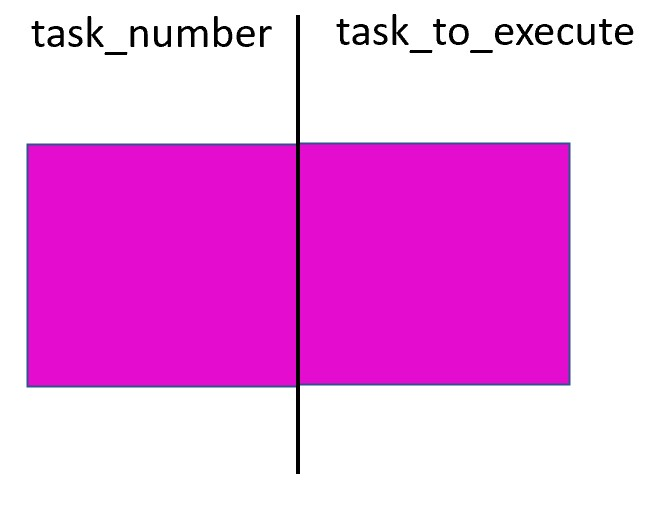
\includegraphics[width=0.5\textwidth]{Pictures/Case1.jpg}
  \caption{Case 1}
  \label{fig: Case 1}
\end{figure}

\smallskip
\noindent
It is the case when the job executed at time t-1 is the same as the job executed a time t (see line 18 - 19 in the algorithm). It is the easiest case. Indeed, we just need to increment the duration of the execution of job because the job will be executed one more unit of time. 


\newpage

\subsubsection{Case 2}

\begin{figure}[h!]
  \centering
  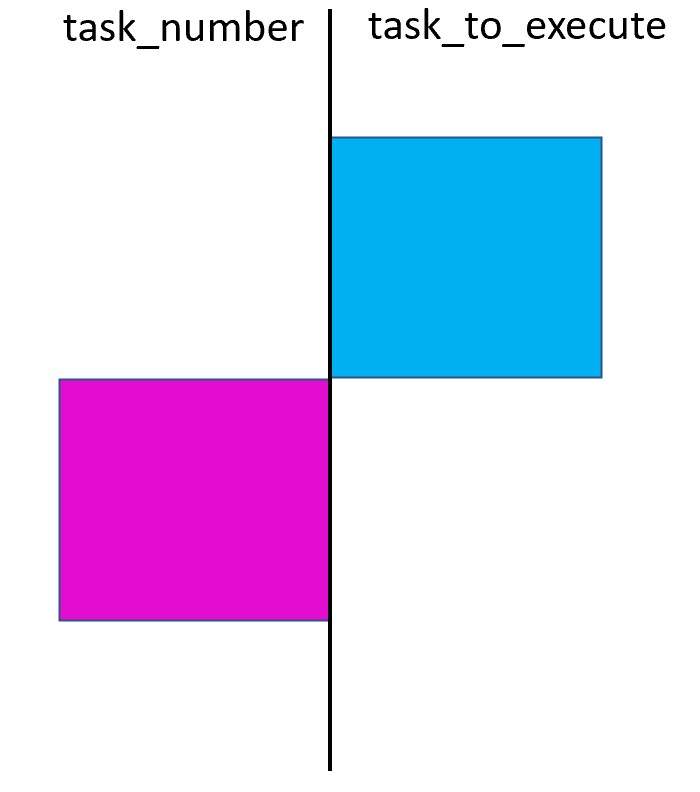
\includegraphics[width=0.5\textwidth]{Pictures/Case2.jpg}
  \caption{Case 2}
  \label{fig: Case 2}
\end{figure}

\smallskip
\noindent
It is the case when at time t-1 the job of a task is executed and at time t the job of another task is executed (see line 12 - 14 in the algorithm). In this case, we add a tuple composed of the start time of the job (given by the variable \textbf{job\_start}) and its duration (given by the variable \textbf{job\_duration}) in a list belonging to the task whose the job was executed at time t-1 (line 12 : ``self.tasks\_list[task\_number - 1].schedule\_solution.append((job\_start,job\_duration))''). We reset the value of the two variables (\textbf{job\_start} = time and \textbf{job\_duration} = 0) for the job which will be executed at time t. 

\newpage
\subsubsection{Case 3}

\begin{figure}[h!]
  \centering
  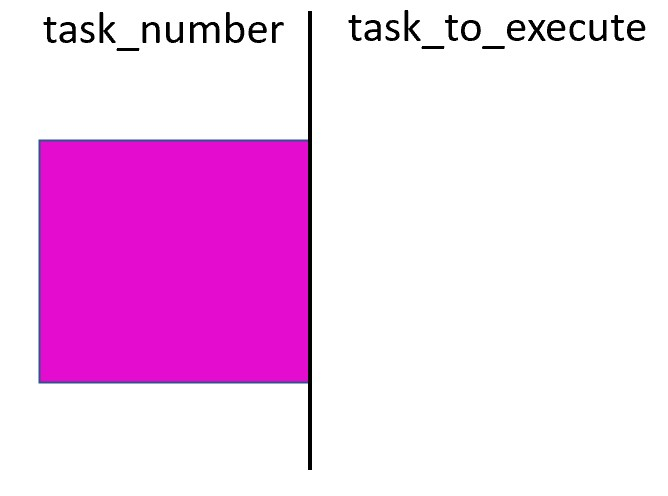
\includegraphics[width=0.5\textwidth]{Pictures/Case3.jpg}
  \caption{Case 3}
  \label{fig: Case 3}
\end{figure}

\smallskip
\noindent
It is the case when a time t-1 the job of a task ended and a time t, there is no tasks that can execute their job (see line 24 -26 in the algorithm). So the value of \textbf{task\_number} is the task number which has its job executed at time t-1 and \textbf{task\_to\_execute} is -1 (because no tasks can execute their job). In this case, we add a tuple composed of the start time of the job (given by the variable \textbf{job\_start}) and its duration (given by the variable \textbf{job\_duration}) in a list belonging to the task whose the job was executed at time t-1 (line 12 : ``self.tasks\_list[task\_number - 1].schedule\_solution.append((job\_start,job\_duration))''). We also set the values of \textbf{job\_duration} and \textbf{job\_start} at 0.

\subsubsection{Case 4}

\begin{figure}[h!]
  \centering
  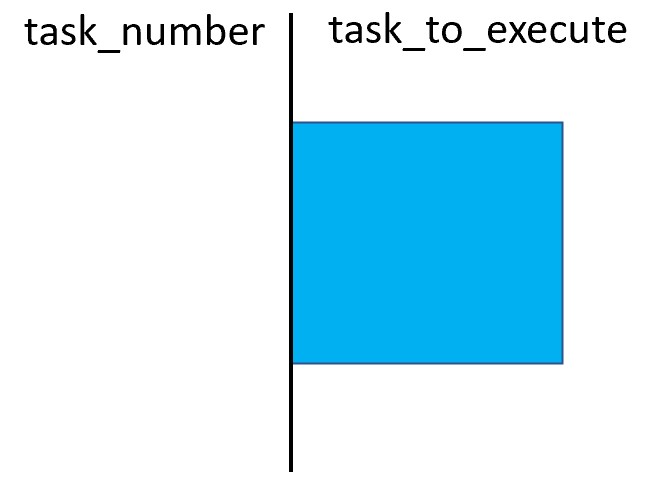
\includegraphics[width=0.5\textwidth]{Pictures/Case4.jpg}
  \caption{Case 4}
  \label{fig: Case 4}
\end{figure}

\smallskip
\noindent
It is the case when no job is executed at time t-1 (it means that the value of \textbf{task\_number = -1}) and a job can be executed a time t (it means that the value of \textbf{task\_to\_execute} is the number of the task which can execute its job). We just need to set the values of \textbf{job\_start} at time t and \textbf{job\_duration} at 1 (see line 16-17 in the algorithm) because a new job starts its execution.

\subsubsection{Case 5}
If the values of \textbf{task\_number} and \textbf{task\_to\_execute} are -1, we do nothing (see line 22 in the algorithm). 

\newpage
\subsection{Result of an execution}

Consider that we have four tasks to schedule and they are ordered by priority : \\

\smallskip
\begin{center}
\begin{tabular}{| l |}
\hline
Task 1 (Offset = 0, WCET = 10, Deadline = 50, Period = 50)\\
Task 2 (Offset = 0, WCET = 20, Deadline = 80, Period = 80)\\
Task 3 (Offset = 0, WCET = 10, Deadline = 100, Period = 100)\\
Task 4 (Offset = 0, WCET = 50, Deadline = 200, Period = 200)\\
\hline
\end{tabular}
\end{center}

\smallskip
\noindent
Thus the priority of the tasks is : Task 1 $>$ Task 2 $>$ Task 3 $>$ Task 4. \\

\noindent
The result of the scheduling is : \\

\begin{figure}[h!]
  \centering
  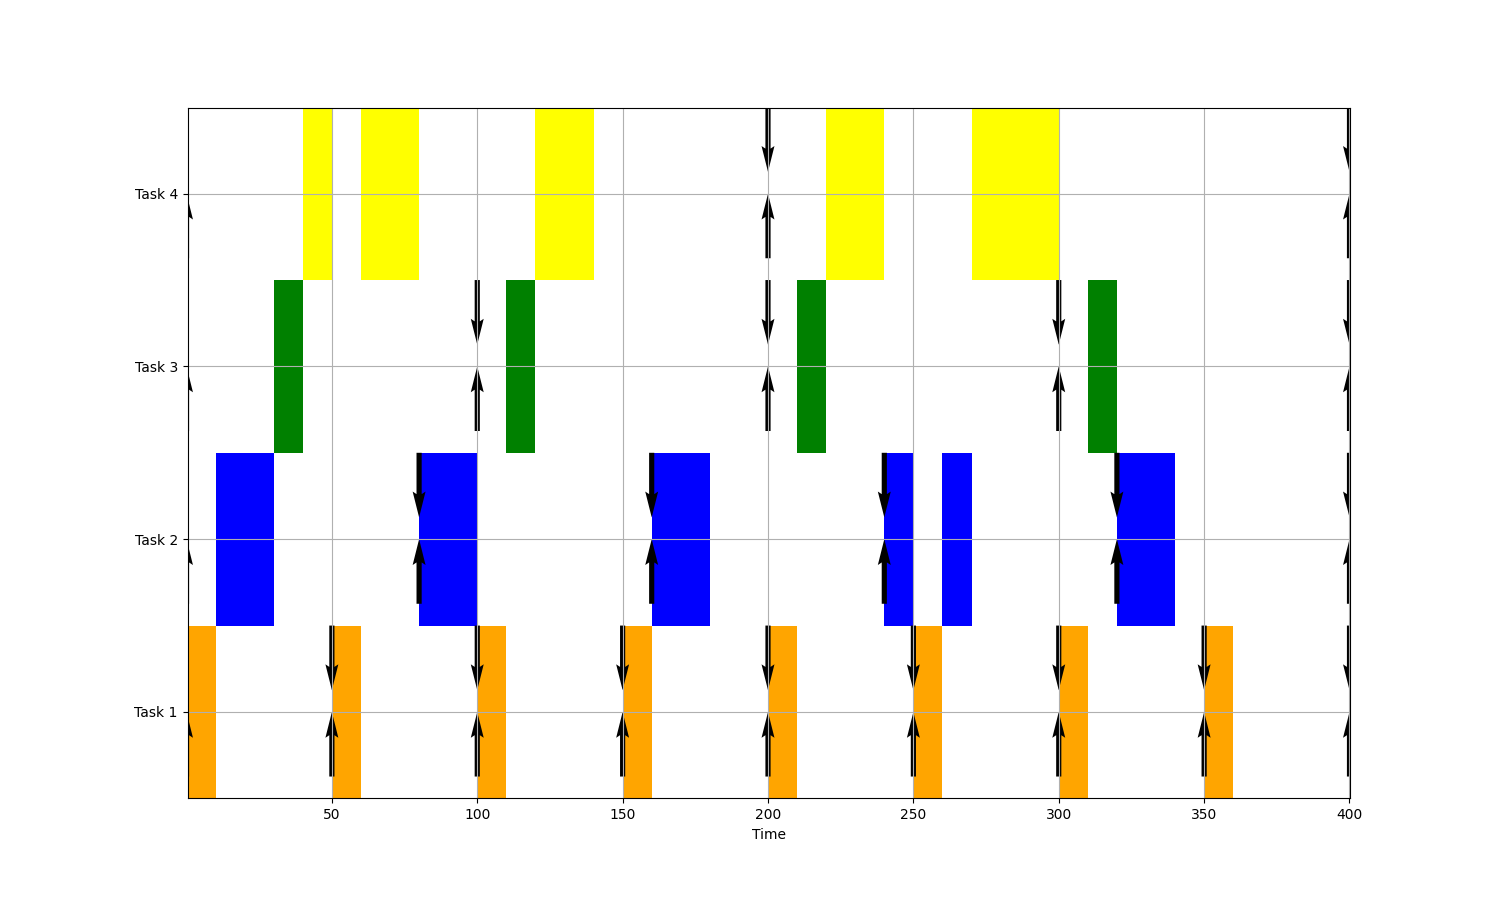
\includegraphics[width=1.25\textwidth]{Figure_1.png}
  \caption{Scheduling 1}
  \label{fig: Scheduling 1}
\end{figure}
\noindent
The arrow $\downarrow$ is when a job can start its execution and the arrow $\uparrow$ is the deadline of a job. 

\newpage 
\noindent
But what happens if a deadline is missed ? Consider the following task : \\
\begin{center}
\begin{tabular}{| l |}
\hline
Task 1 (Offset = 0, WCET = 30, Deadline = 25, Period = 60)\\
\hline
\end{tabular}
\end{center}
This task will always miss its deadline. The result of the scheduling is :\\

\begin{figure}[h!]
  \centering
  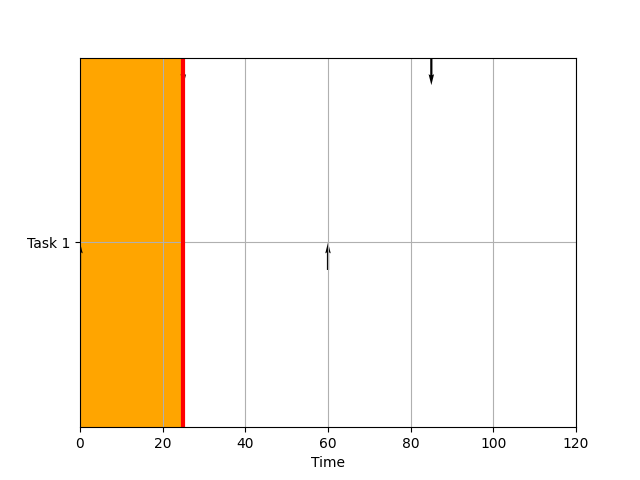
\includegraphics[width=1\textwidth]{Figure_2.png}
  \caption{Scheduling 2}
  \label{fig: Scheduling 2}
\end{figure}
\noindent
 The read line shows that the deadline is missed. 
 
\newpage
\section{Audsley’s priority assignment}

\newpage

\section{Difficulties}

\newpage

\section{Conclusion}

\end{document}